\documentclass[letter]{article}

\usepackage{fullpage}
\usepackage{url}

\title{Performance investigation}

\usepackage[pdftex]{graphicx}
\usepackage{multirow}

\begin{document}
\maketitle

\section{Disjoint set}

Test Id = 3 512 pairs communication of 64 source nodes [0-63] to 512 destination nodes [512-1023]. Each source node sends data to 4 destination nodes e.g rank 0 sends data to ranks 512, 513, 514, 515. 1 rank per node, message size = 8MB. Total data amount transferred is 4GB = 512 x 8 MB. Chunk size for OPTIQ is 64 KB.

\section{Subset tests}

Test Id = 87. Partition size 512.

Number of hops and load - num of paths sharing a physical link.

\begin{center}
    \begin{tabular}{ | l | p{0.75cm} | p{1cm} | p{0.75cm} | p{0.75cm} | p{0.5cm} | p{0.5cm} | p{0.5cm} | p{0.5cm} | p{0.75cm} | p{0.9cm} | p{0.5cm} | p{0.5cm} | p{0.5cm} | p{0.5cm} |}
    \hline
    \multirow{3}{*}{Type} & \multicolumn{2}{ c| }{Performance} &  & \multicolumn{5}{ c| }{Num. of Hops} & \multicolumn{6}{ c| }{Load (Num of Paths)} \\ \cline{2-15}
    & & & & \multirow{2}{1cm}{Total hops} & \multicolumn{4}{ c| }{Per Path} & & & \multicolumn{4}{ c| }{Per Link} \\ \cline{6-15}
    & Time (us) & BW (MB/s) & Num. Paths & & Max & Min & Avg & Med & Total load & Loaded links & Max & Min & Avg & Med \\ \hline
    OPT &  24524 & 83510 & 621 & 3099 & 8 & 1 & 4.99 & 5 & 3099 & 1201 & 9 & 1 & 2.58 & 2\\ \hline
    HEU &  28765 & 71197 & 397 & 1863 & 8 & 1 & 4.69 & 5 & 1863 & 1030 & 3 & 1 & 1.81 & 2\\ \hline
    MPI &  42837 & 47808 & 256 & 1024 & 8 & 1 & 4.00 & 4 & 1024 & 384 & 6 & 1 & 2.67 & 2\\ \hline
    \end{tabular}
\end{center}

Number of copies and load - actual amount of data passing through a link.

\begin{center}
    \begin{tabular}{ | l | p{0.75cm} | p{1cm} | p{0.75cm} | p{0.5cm} | p{1cm} | p{0.5cm} | p{1.5cm} | p{1.25cm} | p{1.25cm} |  p{1.25cm} |}
    \hline
     &  \multicolumn{2}{ c| }{Performance} & \multicolumn{4}{ c| }{Num. of Copies/Node} & \multicolumn{4}{ c| }{Actual Load (Data Amount) per Link} \\ \hline
    Type & Time (us) & BW (MB/s) & Max & Min & Avg & Med & Max & Min & Avg & Med \\ \hline
    OPT & 24524 & 83510 & 1218 & 4 & 397.80 & 301 & 15597568 & 65536 & 8376830 & 7929856 \\ \hline
    HEU & 28765 & 71197 & 1472 & 32 & 400.90 & 320 & 25165824 & 2097152 & 9224144 & 8388608 \\ \hline
    MPI &  42837 & 47808 & & & & & 16777216 & 8388608 & 8388608 & 8388608 \\ \hline
    \end{tabular}
\end{center}

Test Id = 87. Paritition size 2048. 128 sources node sends data to 1024 destination nodes. 8 MB of data for each pair of communication.

\begin{figure}[!htb]
\vspace{-0.1in}
\centering
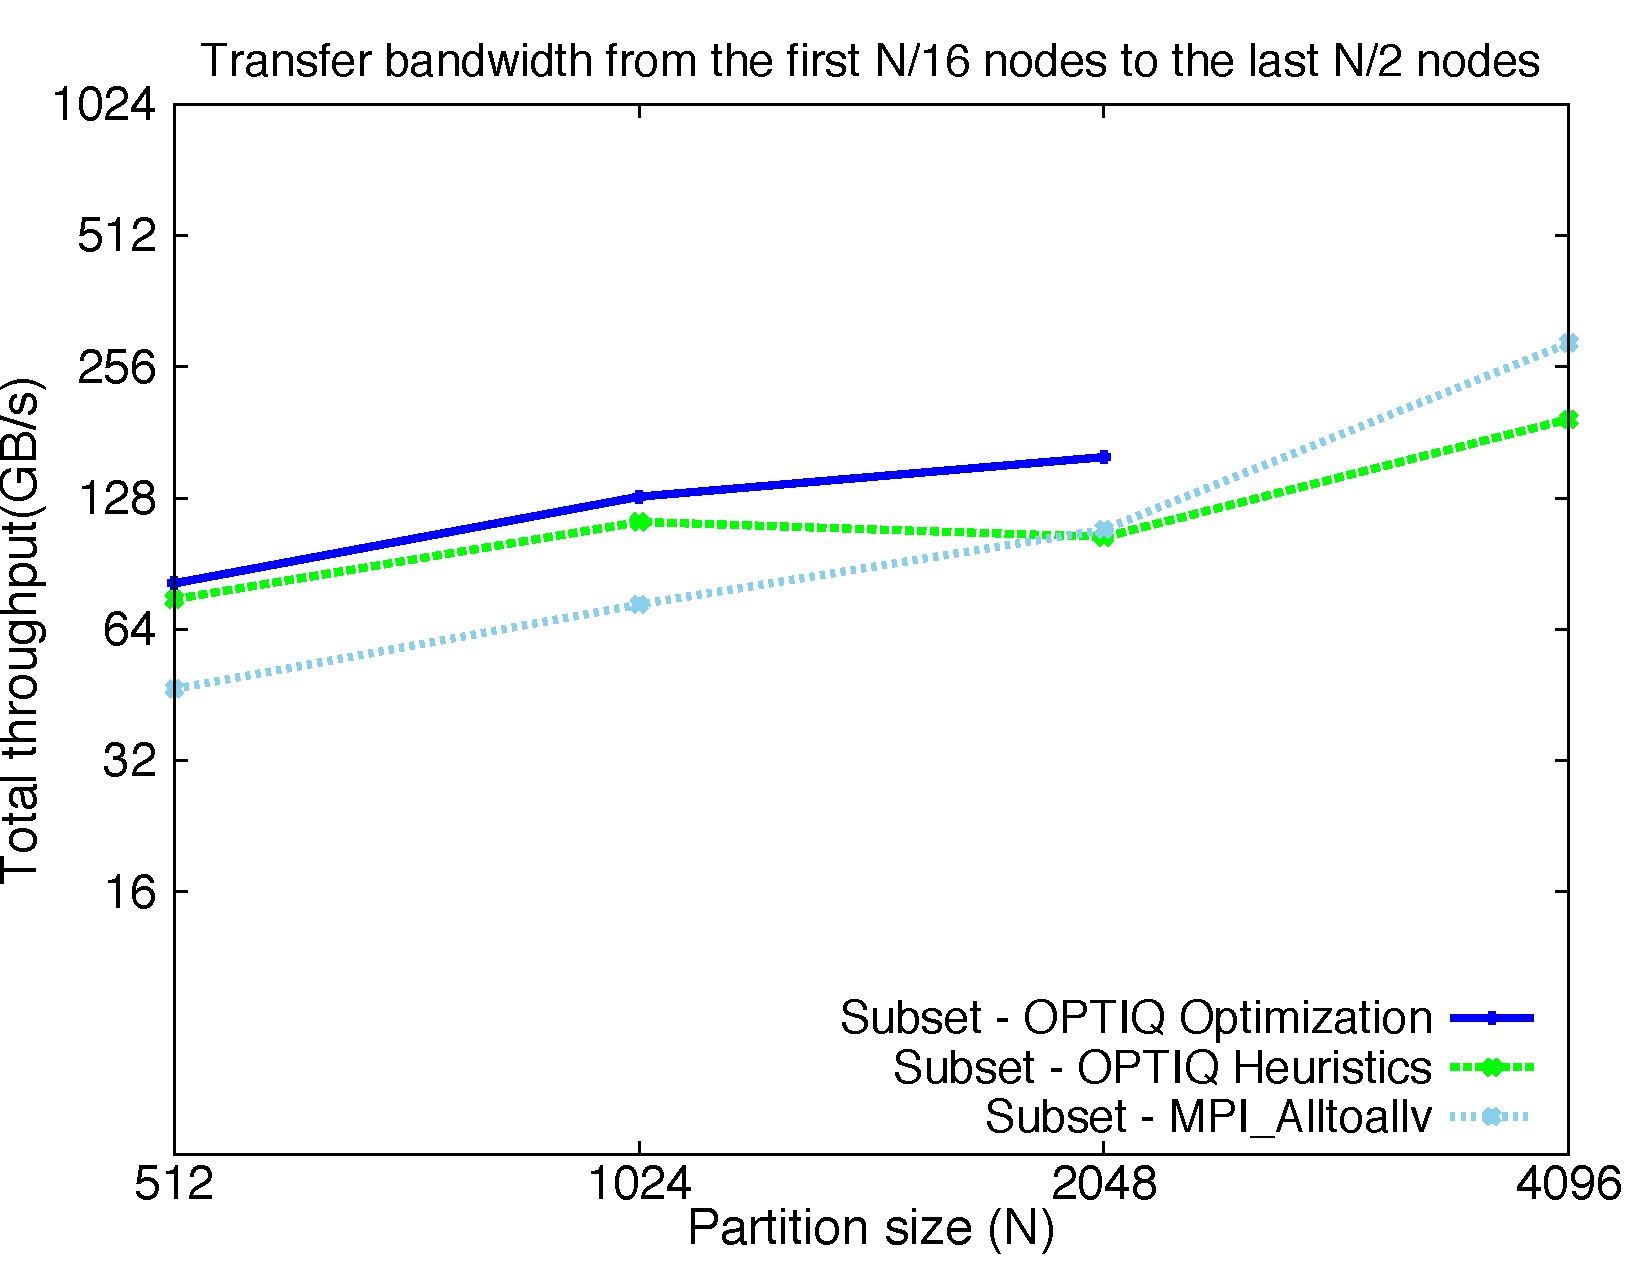
\includegraphics[scale=0.30]{report_figures/constantr_subset.pdf}
\vspace{-0.1in}
\caption{Communication patterns}
\vspace{-0.1in}
\label{fig:patterns}
\end{figure}

\begin{center}
    \begin{tabular}{ | l | p{0.75cm} | p{1cm} | p{0.75cm} | p{0.75cm} | p{0.5cm} | p{0.5cm} | p{0.5cm} | p{0.5cm} | p{0.75cm} | p{0.9cm} | p{0.5cm} | p{0.5cm} | p{0.5cm} | p{0.5cm} |}
    \hline
     &  \multicolumn{2}{ c| }{Performance} &  & \multicolumn{5}{ c| }{Num. of Hops} & \multicolumn{6}{ c| }{Load} \\ \hline
    Type & Time (us) & BW (MB/s) & Num. Paths & Total hops & Max & Min & Avg & Med & Total load & Loaded links & Max & Min & Avg & Med \\ \hline
    MPI & 73731 & 111105 & 1024 & 7168 & 14 & 1 & 7.00 & 7 & 7168 & 1448 & 16 & 1 & 4.95 & 5 \\ \hline
    HEU & 76790 & 106680 & 2603 & 18070 & 14 & 1 & 6.94 & 6 & 18070 & 5133 & 7 & 1 & 3.52 & 3 \\ \hline
    OPT & 50339 & 162736 & 2441 & 18843 & 14 & 1 & 7.72 & 8 & 18843 & 5056 & 16 & 1 & 3.73 & 3 \\
    \hline
    \end{tabular}
\end{center}

\end{document}
